%==============================================================================
% Sjabloon poster bachproef
%==============================================================================
% Gebaseerd op document class `a0poster' door Gerlinde Kettl en Matthias Weiser
% Aangepast voor gebruik aan HOGENT door Jens Buysse en Bert Van Vreckem

\documentclass[a0,portrait]{hogent-poster}

% Info over de opleiding
\course{Bachelorthesis}
\studyprogramme{Bachelor of applied computer science}
\academicyear{2024-2025}
\institution{Hogeschool Gent, Valentin Vaerwyckweg 1, 9000 Gent}

% Info over de bachelorproef
\title{Accessible Password Management Using Face Recognition for Individuals with Cognitive and Motor Disabilities}
\subtitle{Ondertitel (eventueel)}
\author{Abdellah El Halimi}
\email{abdellah.elhalimimerroun@student.hogent.be}
\supervisor{Dhr. A. De Witte}
\cosupervisor{Dhr. C. Dutoict}

% Indien ingevuld, wordt deze informatie toegevoegd aan het einde van de
% abstract. Zet in commentaar als je dit niet wilt.
\specialisation{Full Stack Development}
\keywords{Face Recognition, Password Management, Cognitive Disabilities, Motor Disabilities}
\projectrepo{https://github.com/user/repo}

\begin{document}

\maketitle

\begin{abstract}
This poster presents a web-based password manager that uses facial recognition to authenticate users with cognitive and motor disabilities. The system encrypts user passwords in the browser and stores them securely on the server. It uses face recognition to verify user identity and provides a user-friendly interface for managing passwords. The system is designed to be accessible and easy to use for individuals with cognitive and motor disabilities.
\end{abstract}

\begin{multicols}{2} % This is how many columns your poster will be broken into, a portrait poster is generally split into 2 columns

\section{Introductie}

In today's digital age, authentication is a crucial element of cybersecurity. Traditional password-based systems require users to create, remember, and accurately enter complex passwords. For individuals with cognitive or motor disabilities, this process presents significant challenges that can lead to frustration, frequent lockouts, and increased security risks.

The increasing reliance on online services has amplified the need for secure and accessible authentication solutions. Conventional methods often fail to accommodate the unique needs of users with disabilities. Cognitive impairments may hinder memory recall, while motor disabilities can complicate the physical act of typing.

This research explores the integration of face recognition technology into a password manager to develop an accessible and user-friendly authentication method. The implementation leverages \texttt{face-api.js} for lightweight browser-based face detection, \texttt{TypeScript} for enhanced code reliability, \texttt{SQLite} for local credential storage, and \texttt{bcrypt} for secure password hashing.

\section{Experimenten}

A newt? Camelot! Why? No, no, no! Yes, yes. A bit. But she's got a wart.

Shut up! I dunno. Must be a king. Who's that then? Look, my liege! On second thoughts, let's not go there. It is a silly place.

Shut up! Will you shut up?! No, no, no! Yes, yes. A bit. But she's got a wart. He hasn't got shit all over him. It's only a model. It's only a model.

Bring her forward! I don't want to talk to you no more, you empty-headed animal food trough water! I fart in your general direction! Your mother was a hamster and your father smelt of elderberries! Now leave 

\section{Sectie met figuur}

De {\LaTeX} figure-omgeving bepaalt zelf waar een afbeelding komt en dat is meestal niet op de plek in de tekst waar de figure-omgeving gedefinieerd wordt. Als je wilt forceren dat afbeeldingen toch in de flow van de tekst blijven, dan kan je dat zoals hieronder:

\begin{center}
  \captionsetup{type=figure}
  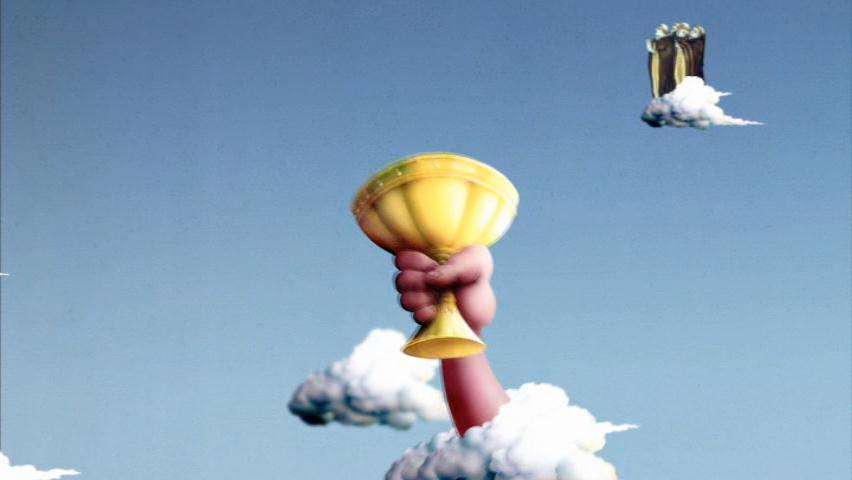
\includegraphics[width=1.0\linewidth]{grail}
  \captionof{figure}{He hasn't got shit all over him. The nose? Where'd you get the coconuts? What do you mean? We shall say `Ni' again to you, if you do not appease us}
\end{center}

Let er wel op dat dit tot problemen met bladschikking kan leiden.

\section{Conclusies}

Don't underestimate the Force. Oh God, my uncle. How am I ever gonna explain this? I suggest you try it again, Luke. This time, let go your conscious self and act on instinct. Don't be too proud of this technological terror you've constructed. The ability to destroy a planet is insignificant next to the power of the Force.

\section{Toekomstig onderzoek}

I care. So, what do you think of her, Han? No! Alderaan is peaceful. We have no weapons. You can't possibly… I have traced the Rebel spies to her. Now she is my only link to finding their secret base.

Kid, I've flown from one side of this galaxy to the other. I've seen a lot of strange stuff, but I've never seen anything to make me believe there's one all-powerful Force controlling everything. There's no mystical energy field that controls my destiny. It's all a lot of simple tricks and nonsense. You are a part of the Rebel Alliance and a traitor! Take her away! 

\end{multicols}
\end{document}